\vspace*{-5mm}
\begin{enumerate}
\item[11] The limiter must have 4 bands.
\item[12] The bands of the limiter must comply with the class 2 of IEC 6964 standard (2001). 
\item[13] The limiters must apply to frequencies below 500 Hz.
\end{enumerate}

\vspace*{-5mm}
A filter for decimation will be designed which must meet requirement 12, and a filter for interpolation will be designed which must not influence the decimated signals bandwidth, because it would otherwise influence the frequency response of the system making it non linear. The decimation filter will be deigned first.

Because the system is a multirate system with octave bands as mentioned in \autoref{ch:designRealization} only one filter needs to be designed because the sampling frequency is halved for every octave resulting in the same coefficients for all decimation and interpolation filters.

\section{Decimation Filter}\label{sec:decFilter}
The decimation filter must meet requirement 12 as just mentioned which states the requirements for the filter. The requirements can be seen in \autoref{fig:band1_reqOverview} and \autoref{tb:normalizedReqClass2} which states the requirements to the figure.

\begin{figure}[H]
\centering
\begin{subfigure}[t]{0.45\textwidth}
	\tikzsetnextfilename{Band1Req}
	% This file was created by matlab2tikz.
%
%The latest updates can be retrieved from
%  http://www.mathworks.com/matlabcentral/fileexchange/22022-matlab2tikz-matlab2tikz
%where you can also make suggestions and rate matlab2tikz.
%
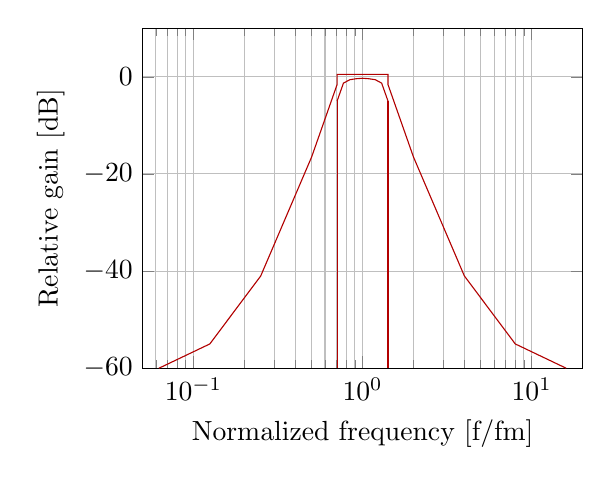
\begin{tikzpicture}

\begin{axis}[%
width=2.2in,
height=1.7in,
at={(0.758in,0.481in)},
scale only axis,
unbounded coords=jump,
xmode=log,
xmin=0.05,
xmax=20,
xminorticks=true,
xlabel={Normalized frequency [f/fm]},
xmajorgrids,
xminorgrids,
ymin=-60,
ymax=10,
ylabel={Relative gain [dB]},
ymajorgrids,
axis background/.style={fill=white}
]
\addplot [color=black!30!red,solid,forget plot]
  table[row sep=crcr]{%
1.4142	-5\\
1.4142	-60\\
};
\addplot [color=black!30!red,solid,forget plot]
  table[row sep=crcr]{%
0.7071	-5\\
0.7071	-60\\
};
\addplot [color=black!30!red,solid,forget plot]
  table[row sep=crcr]{%
0.0625	-60\\
0.125	-55\\
0.25	-41\\
0.5	-16.5\\
0.707106781186547	-1.6\\
0.707106781186547	0.5\\
0.77110541270397	0.5\\
0.840896415253715	0.5\\
0.917004043204671	0.5\\
1	0.5\\
1.09050773266526	0.5\\
1.18920711500272	0.5\\
1.29683955465101	0.5\\
1.4142135623731	0.5\\
1.4142135623731	-1.6\\
2	-16.5\\
4	-41\\
8	-55\\
16	-60\\
};
\addplot [color=black!30!red,solid,forget plot]
  table[row sep=crcr]{%
0.0625	-inf\\
0.125	-inf\\
0.25	-inf\\
0.5	-inf\\
0.707106781186547	-5\\
0.707106781186547	-5\\
0.77110541270397	-1.3\\
0.840896415253715	-0.6\\
0.917004043204671	-0.4\\
1	-0.3\\
1.09050773266526	-0.4\\
1.18920711500272	-0.6\\
1.29683955465101	-1.3\\
1.4142135623731	-5\\
1.4142135623731	-5\\
2	-inf\\
4	-inf\\
8	-inf\\
16	-inf\\
};
\end{axis}
\end{tikzpicture}%
	\caption{Band requirements.}
	\label{fig:band1_req}
\end{subfigure}
\begin{subfigure}[t]{0.45\textwidth}
	\tikzsetnextfilename{Band1ReqZoom}
	% This file was created by matlab2tikz.
%
%The latest updates can be retrieved from
%  http://www.mathworks.com/matlabcentral/fileexchange/22022-matlab2tikz-matlab2tikz
%where you can also make suggestions and rate matlab2tikz.
%
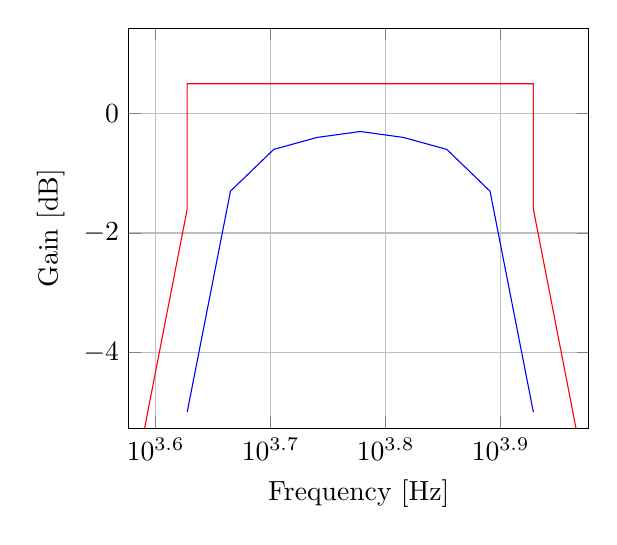
\begin{tikzpicture}

\begin{axis}[%
width=2.3in,
height=2in,
at={(0.758in,0.504in)},
scale only axis,
unbounded coords=jump,
xmode=log,
xmin=3774.50218155918,
xmax=9480.85426960068,
xminorticks=true,
xlabel={Frequency [Hz]},
xmajorgrids,
xminorgrids,
ymin=-5.26838030133928,
ymax=1.43014090401786,
ylabel={Gain [dB]},
ymajorgrids,
axis background/.style={fill=white}
]
\addplot [color=red,solid,forget plot]
  table[row sep=crcr]{%
375	-60\\
750	-55\\
1500	-41\\
3000	-16.5\\
4242.64068711928	-1.6\\
4242.64068711928	0.5\\
4626.63247622382	0.5\\
5045.37849152229	0.5\\
5502.02425922803	0.5\\
6000	0.5\\
6543.04639599155	0.5\\
7135.24269001633	0.5\\
7781.03732790606	0.5\\
8485.28137423857	0.5\\
8485.28137423857	-1.6\\
12000	-16.5\\
24000	-41\\
48000	-55\\
96000	-60\\
};
\addplot [color=blue,solid,forget plot]
  table[row sep=crcr]{%
375	-inf\\
750	-inf\\
1500	-inf\\
3000	-inf\\
4242.64068711928	-5\\
4242.64068711928	-5\\
4626.63247622382	-1.3\\
5045.37849152229	-0.6\\
5502.02425922803	-0.4\\
6000	-0.3\\
6543.04639599155	-0.4\\
7135.24269001633	-0.6\\
7781.03732790606	-1.3\\
8485.28137423857	-5\\
8485.28137423857	-5\\
12000	-inf\\
24000	-inf\\
48000	-inf\\
96000	-inf\\
};
\end{axis}
\end{tikzpicture}%
	\caption{Band requirements zoomed in.}
	\label{fig:band1_reqZoom}
\end{subfigure}
\caption{Band requirements without and with zoom.}
\label{fig:band1_reqOverview}
\end{figure}


\begin{table}[H]
\centering
\begin{tabular}{|c|c|}
\hline
\multirow{3}{*}{\begin{tabular}[c]{@{}c@{}}Normalized\\ frequency\\ $f/f_m=\Omega$\end{tabular}}                        & \begin{tabular}[c]{@{}c@{}}Minimum;Maximum attenuation limits\\ dB\end{tabular}                        \\ \cline{2-2} 
                                                                                                                        & Filter class                                                                                           \\ \cline{2-2} 
                                                                                                                        & 2                                                                                                      \\ \hline
$G^0$                                                                                                                   & -0,5;+0,5                                                                                              \\ \hline
$G^{\pm 1/8}$                                                                                                           & -0,5; +0,6                                                                                             \\ \hline
$G^{\pm 1/4}$                                                                                                           & -0,5; +0,8                                                                                             \\ \hline
$G^{\pm 3/8}$                                                                                                           & -0,5; +1,6                                                                                             \\ \hline
$<G^{\pm 1/2}$                                                                                                          & -0,5; +5,5*                                                                                            \\ \hline
$>G^{\pm 1/2}$                                                                                                          & +1,6; +5,5*                                                                                            \\ \hline
$G^{\pm 1}$                                                                                                             & +16,5; +$\infty$                                                                                       \\ \hline
$G^{\pm 2}$                                                                                                             & +41; +$\infty$                                                                                         \\ \hline
$G^{\pm 3}$                                                                                                             & +55; +$\infty$                                                                                         \\ \hline
$\geq G^{\pm +4}$                                                                                                       & +60; +$\infty$                                                                                         \\ \hline
$\leq G^{\pm -4}$                                                                                                       & +60; +$\infty$                                                                                         \\ \hline
\multicolumn{2}{|l|}{\begin{tabular}[c]{@{}l@{}}* At frequencies less than the lower band-edge frequency and greater than the\\ upper band-edge frequency, the limit on maximum relative attenuation is +$\infty$;\end{tabular}} \\ \hline
\end{tabular}
\caption{Normalized requirements for the filters. G=2.}
\label{tb:normalizedReqClass2}
\end{table} 
 
Only a lowpass filter should be designed because of spectral inversion, as described in \autoref{ch:designRealization}, so instead of bandpass requirements only one side of the requirements are shown from now on. %From system overview the octave bands are given for frequencies below 530 Hz, see \autoref{tb:freqBands} which meets requirement 8 and 10.
